% Fibers of the trivial line bundle: the preimage of each point is a line.
% Source: book/tex/riemann-surface/line-bundles.tex (asy figure).
\documentclass[border=2mm]{standalone}
\usepackage{tikz}
\begin{document}
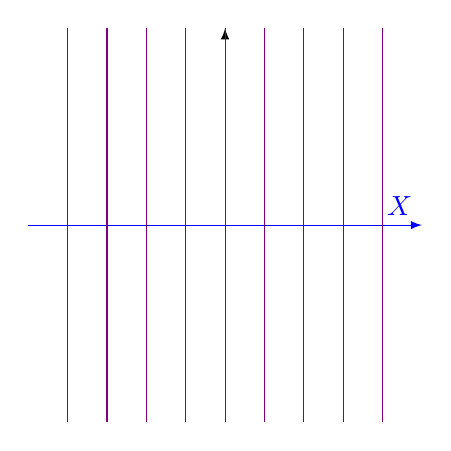
\begin{tikzpicture}[scale=0.5,>=latex]
  \draw[blue,->] (-5,0) -- (5,0) node[anchor=south east] {$X$};
  \draw[->] (0,-5) -- (0,5);
  \draw[violet] (-4,-5) -- (-4,5);
  \draw[violet] (-3,-5) -- (-3,5);
  \draw[violet] (-2,-5) -- (-2,5);
  \draw[violet] (-1,-5) -- (-1,5);
  \draw[violet] (0,-5) -- (0,5);
  \draw[violet] (1,-5) -- (1,5);
  \draw[violet] (2,-5) -- (2,5);
  \draw[violet] (3,-5) -- (3,5);
  \draw[violet] (4,-5) -- (4,5);
\end{tikzpicture}
\end{document}
